\section{Konzept}
Die Auftraggeber verlangen ein Gerät das folgenden Anforderungen gerecht werden soll. Die Anforderungen wurden dem Pflichtenheft entnommen, welches sich im Anhang befindet.
\begin{itemize}
\item Das Messgerät muss mit den SEV 1011 Steckverbinder kompatibel sein.
\item Durch ein Kunststoffgehäuse muss die Schutzart IP 20 gewahrleistet werden.
\item Wenn das Gerät nicht der Schutzklasse 2 entspricht muss eine  Potenzialtrennung vorhanden sein.
\item Die Peripherie enthält im Minimum ein Status LED und ein Reset-Schalter.
\item Die Messung muss für U=360V und I=15A (Netzspannung) ausgelegt sein.
\item Messbereiche: bis 0.5A; 0.5 bis 5A; 5 bis 15A
\item Auflösung: bis 1A $\pm$ 2W; bis 10A $\pm$ 20W
\item Harmonische Schwingungen bis 5kHz mussen detektiert werden.
\item Der Log Intervall der Leistung muss 10s sein.
\item Firmware für die Signalwandlung, Leistungsberechnung, Datenspeicherung und den Transfer zum Empfangsgerät.
\item Es muss eine Software mitgeliefert werden, welche den Empfang und die Darstellung des Leistungsgerätes sicherstellt.
\item Die Daten werden über Bluetooth an eine Computer-Applikation gesendet, welcher als Empfänger dient.
\end{itemize}
Aus diesen Anforderungen wurden die folgenden Konzepte abgeleitet.

\subsection{Mechanischer Aufbau}
Der mechanische Aufbau ist durch das Printdesign geprägt. P3T7 besteht aus einem \\ ATmega2560-Board, welches mit 2 «Shields» bestückt wurde. Auf dem obersten Layer befinden sich unter anderem die benötigten Messshunts, der Spannungsteiler, das Netzteil für die $\pm 5V$ Versorgung sowie Sicherungen, welche bei zu hohen Strömen auslösen. Auf dem 2. Layer werden die Messsignale aufbereitet und anschliessend an den Mikrocontroller weitergeben. Das Mikrocontrollerboard ist mit den Massen 54 x 100 der kleinste Layer und wird vom zweiten Print (90 x 125) komplett «verdeckt». Der oberste Print ist um 20 mm seitwärts zum zweiten Layer versetzt und zudem 5 mm schmäler. Durch dies kann durch Distanzbolzen im Gehäuse der Print befestigt werden. Das Gehäuse besitzt eine Kabelverschraubung, durch welche ein SEV 1011 Stecker Typ 12 befestigt ist. Auf der entgegengesetzten Seite können Verbraucher über eine SEV 1011 Steckdose angeschlossen werden.
Das Gehäuse wird durch 4 Schrauben geschlossen. Durch das Kunststoffgehäuse werden jegliche Berührungen mit elektrisch leitenden Teilen verhindert. Falls die Sicherung ansprechen sollte, muss das Gerät vom Netz getrennt werden, bevor die Sicherung ausgewechselt werden kann. 


\begin{figure}[H]
\begin{center}
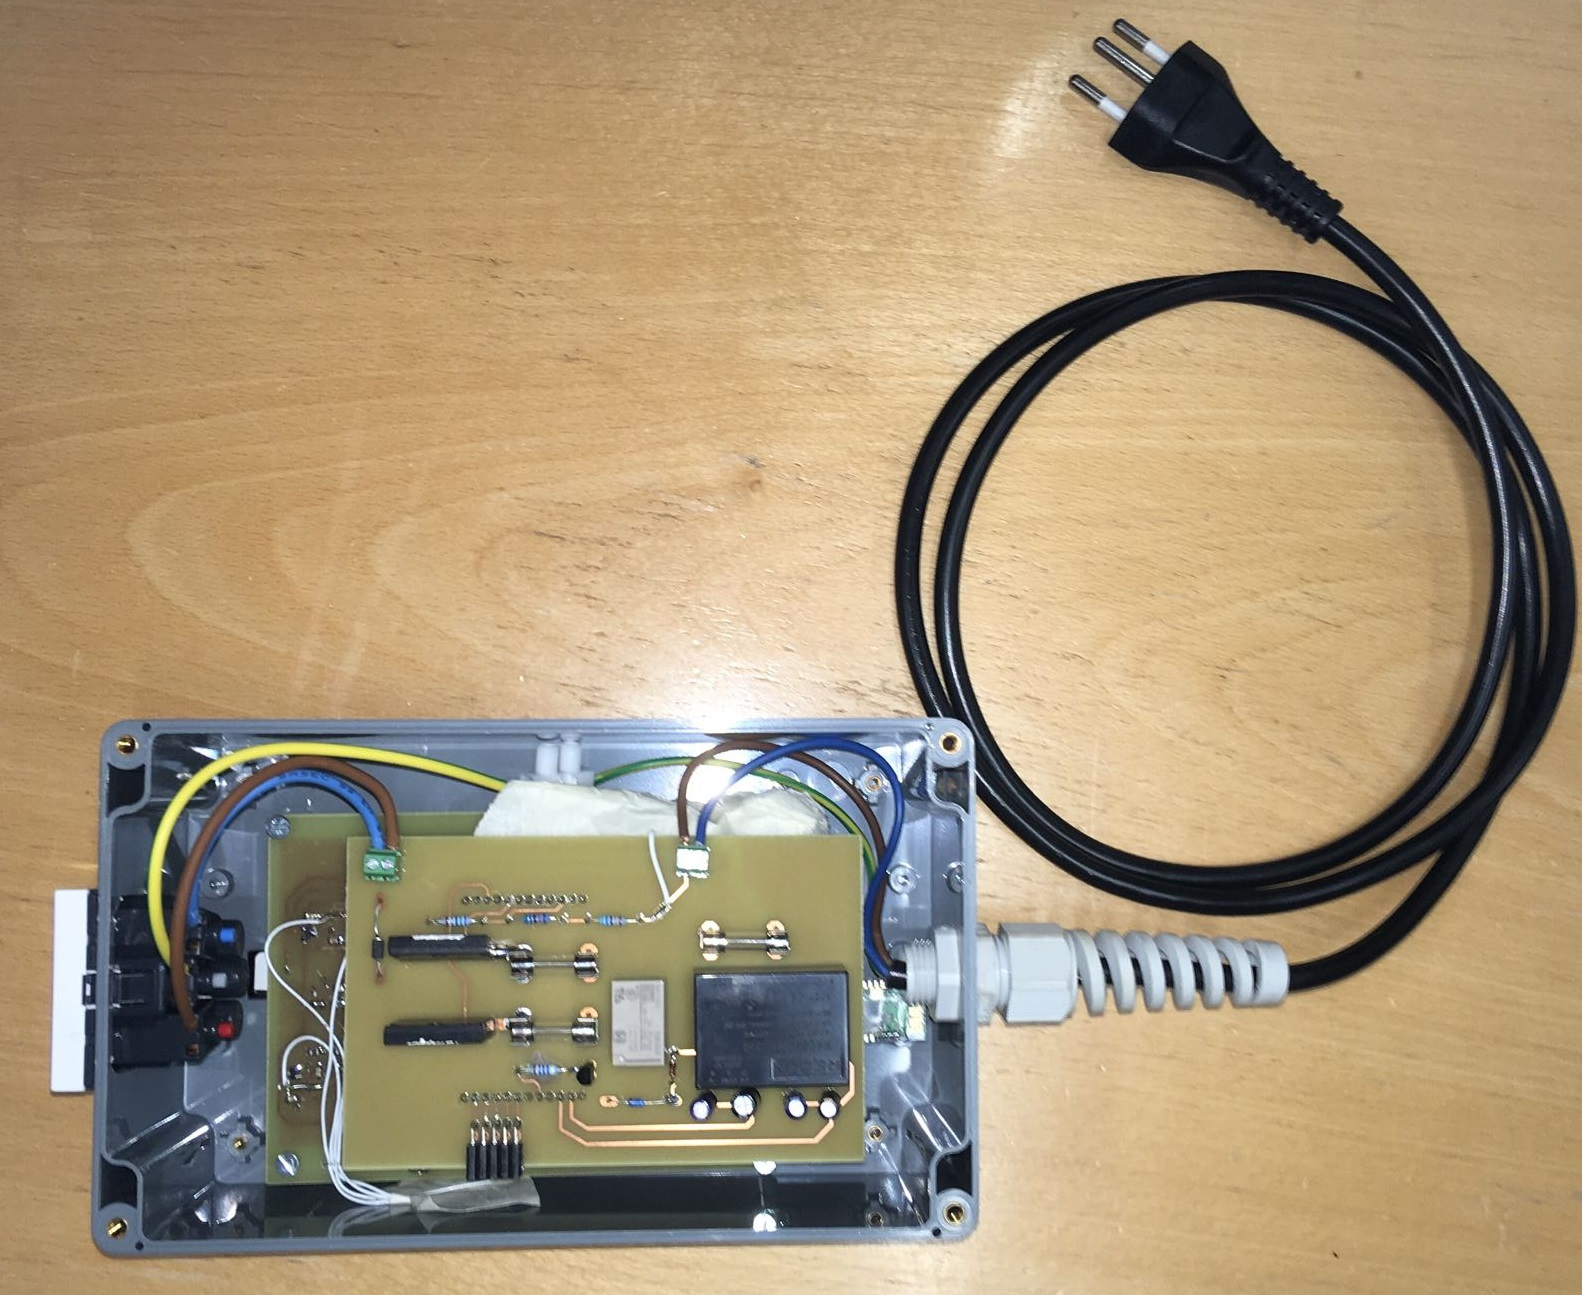
\includegraphics[width=0.7\textwidth ]{images/Konzept_MechAuf.jpeg}
\caption{Mechanischer Aufbau}
\label{fig:Mechanischer_Aufbau}
\end{center}
\end{figure}

\subsection{Elektrischer Aufbau}
Der elektrische Aufbau gliedert sich in vier verschiedene Teile. Auf dem obersten Print wird mit Netzspannung gearbeitet. Auf dem folgenden Print befindet sich der Digitalbereich und der Analogbereich. Im Digitalbereich ist die Verbindung zu den verschiedenen Bauteilen realisiert. Es sind eine Realtimelclock(RTC), ein Flashspeicher und ein Bluetooth-Modul vorhanden. Die RTC wird gebraucht, um einen Zeitstempel den Daten beizugeben. Der Flashspeicher wird verwendet, um Daten über einen längeren Zeitraum zu speichern sowohl als auch um die Daten nicht nicht-flüchtig zu speichern. Und das Bluetooth Modul wird gebraucht, um eine drahtlose Verbindung zum PC herzustellen. Im Analogbereich wird die Signalaufbereitung gemacht, diese wird im Kapitel \ref{sec:analoge_schaltung} behandelt. Die unterste Schicht ist ein Arduino Mega, welcher die Recheneinheit des P3T7 darstellt.

\begin{figure}[H]
\begin{center}
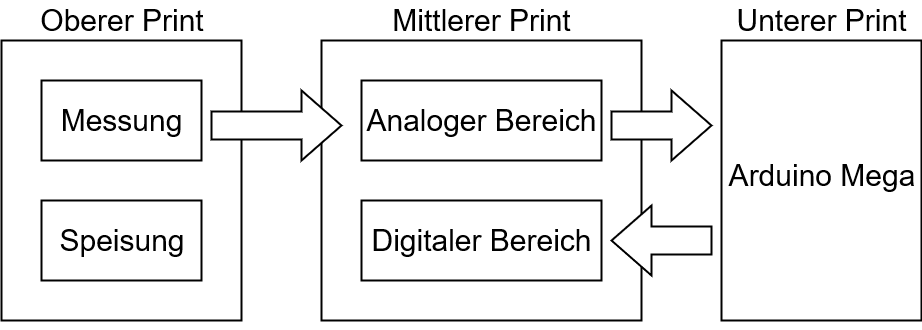
\includegraphics[width=0.9\textwidth]{images/Konzept_Elektrischer_Aufbau.png}
\caption{Konzept Elektrischer Aufbau}
\end{center}
\end{figure}


\subsection{Firmware Aufbau}
Das Messgerät kann drei Betriebszustände unterschieden: dem Echtzeitmodus, dem Übertragungsmodus und dem normalen Modus. Im normalen Modus misst das Messgerät für jeweils 10 Sekunden und speichert die mittlere Leistung zusammen mit einem Zeitstempel auf einen Speicher. Im Echtzeitmodus wird zusätzlich zur Speicherung die mittlere Leistung einmal pro Sekunde auf die Java-Applikation zur Visualisierung übertragen. Befindet sich das Gerät im Übertragungsmodus, wird die Messung temporär deaktiviert, der gesamte Speicher ausgelesen und auf die PC-Software übertragen.

Die Steuerung der Messungen erfolgt durch einen softwaregenerierten Timer, welcher im Hauptprogramm einen Interrupt auslöst. Erfolgt dieser, so wird die Momentanleistung gemessen und das Ergebnis in einem Buffer gespeichert. Bei jedem weiterem Interrupt wird die Leistung erneut gemessen und im Buffer aufsummiert. Die Anzahl an Interrupts wird von der Software gezählt. Nach 10 Sekunden wird die mittlere Leistung berechnet und im Flashspeicher des Messgerätes abgelegt. Abbildung XXX zeigt eine schematische Abbildung des Grobkonzeptes der Firmware.

\begin{figure}[H]
\begin{center}
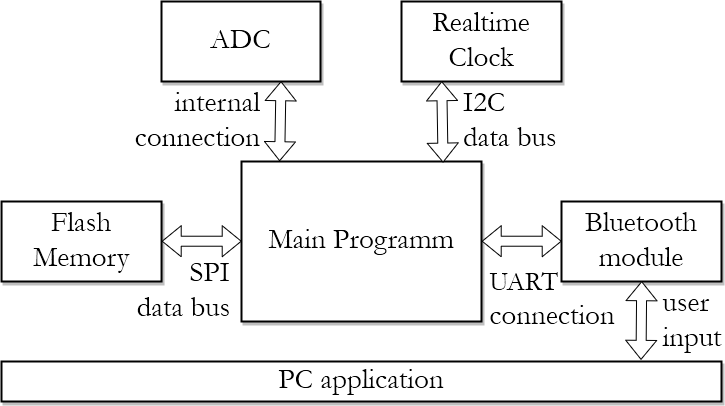
\includegraphics[width=0.7\textwidth ]{images/Konzept_Firmware.png}
\caption{Firmware Aufbau}
\label{fig:Firmware_Aufbau}
\end{center}
\end{figure}

\subsection{Software Aufbau}
Die Software stellt die Schnittstelle zwischen dem Menschen und dem P3T7 dar. Sie hat die Aufgabe die Daten aus dem P3T7 zu lesen und sie für weitere Berechnungen bereitzustellen. Damit die Daten einfach weiterverarbeitbar sind, generiert die Software ein CSV-File. Dieses kann leicht in Excel oder Matlab importiert werden. Des Weitern werden Berechnungen mit der Software gemacht, für welche der Controller zu schwach ist und um Speicherplatz auf dem P3T7 zu sparen.

\begin{figure}[H]
\begin{center}
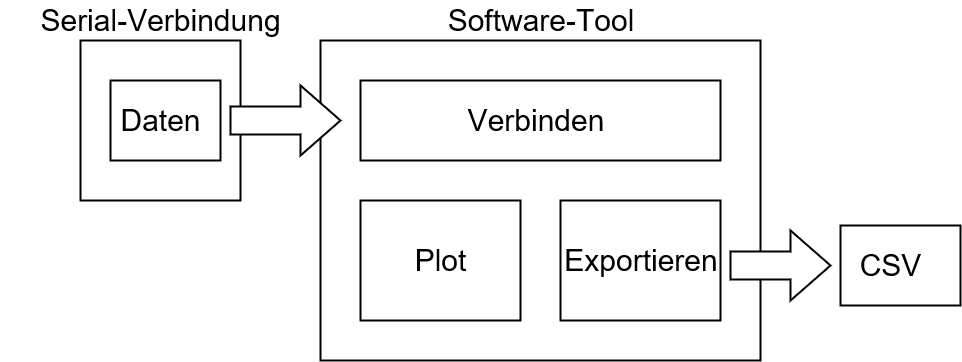
\includegraphics[width=0.9\textwidth]{images/Konzept_Software.png}
\caption{Konzept Software}
\end{center}
\end{figure}

Die Software stellt auch einen Plot mit den ausgelesenen Daten zur Verfügung. Der Plot soll dem User die Möglichkeit geben, die Daten zu validieren, bevor er sie weiterverarbeitet.